\documentclass[a4paper,11pt]{report}
\usepackage[T1]{fontenc}
\usepackage[utf8]{inputenc}
\usepackage[polish]{babel}
\usepackage{lmodern}
\usepackage{graphicx}

\title{Roznice w czasie realizacji sortowania metodą quicksort, w zależności od wyboru elementu rozdzielającego}
\author{Arkadiusz Cyktor 200367}

\begin{document}
\maketitle

\begin{figure}
\textbf{Przypadek optymistyczny} dla algorytmu \emph{quicksort}, to sytuacja, w której do podziału tablicy za każdym razem uda nam się wybrać medianę sortowanego fragmentu.
\end{figure}
\begin{figure}
\textbf{Przypadek przeciętny} dla algorytmu \emph{quicksort}, to sytuacja, w której występuje równomierne prawdopodobieństwo wyboru elementu dzielącego.
\end{figure}
\begin{figure}
\textbf{Przypadek pesymistyczny} dla algorytmu \emph{quicksort}, to sytuacja, w której sortujemy uporządkowaną już tablicę.
\end{figure}



\begin{figure}
  1. Poniższy wykres przedstawia zależność czasu potrzebnego na wykonanie algorytmu \textbf{quicksort} dla przypadku przeciętnego. Jak widac jest to funkcja \emph{O(nlogn)}.
\begin{center} 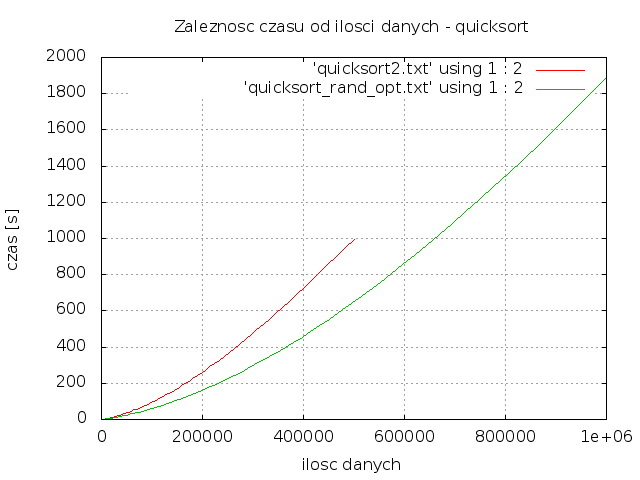
\includegraphics[scale=0.55]{./quicksort_opt.png}\end{center}
   Linia czerwona odpowiada algorytmowi, w którym elementem rozdzielającym zawsze było środkowe pole wektora. Zielona natomoiast, obrazuje zależność dla przypadku, gdy element ten wybierany był losowo.
  \\ Ze względu na długi czas symulacji, pierwszy z wykresów zatrzymuje się na wartości 500000 elementów, jednak nawet w takiej skali widać, że w obu przypadkach złożoność obliczeniowa rośnie w taki sam sposób, drugie z rozwiązań wydaje się być jednak wydajniejsze. Ponieważ w przypadku optymistycznym dla algorytmu quicksort, złożoność obliczeniowa również zmienia się według funkcji \emph{nlogn} (Według literatury jest jednak niższa o około 39 procent - dokładana złożoność dla przypadku przeciętnego wynosi \emph{O(2nln(n)}, co w przybliżeniu wynosi \emph{O(1,39nlogn)}\footnote{1}), wykresy dla niej prezentowałyby się prawie identycznie jak powyższe (co wiąże się z takimi samymi wnioskami), dlatego postanowiłem ich nie zamieszczać. 
  \\
  \\
  1) Obliczenia oparte na informacjach ze strony www.toyoteczka.mainrc.com/pliki/asd/quicksort.pdf
   \end{figure}


\begin{figure}
  2. Ponizszy wykres przedstawia zależność czasu potrzebnego na wykonanie algorytmu od ilości elementów dla przypadku pesymistycznego.
\begin{center}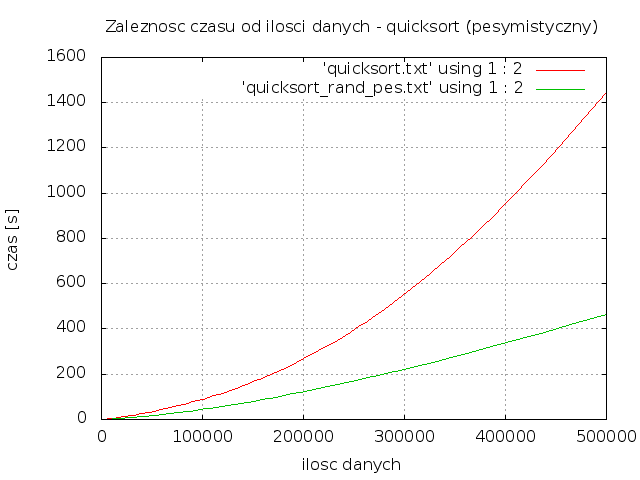
\includegraphics[scale=0.55]{./quicksort_pes.png}\end{center}
    Zielona linia prezentuje zachowanie algorytmu, w którym element rozdzielający wybierany był losowo, natomiast czerwona ten, w którym wybierano element środkowy. Jak widać, dla pierwszego z nich, złożoność jest bardzo zbliżona do tej z przypadku przeciętnego - również rośnie według funkcji \emph{O(nlogn)}. W przypadku drugiego możemy zaobserwować większą zmianę - tutaj złożoność rośnie wykładniczo. Łatwo można dojść więc do wniosku, że losowanie elementu rozdzielającego wpływa bardzo korzystnie na złożoność obliczeniową naszego algorytmu oraz zabezpiecza go przed przypadkiem pesymistycznym.
\end{figure}
\end{document}
